In the last chapter we have introduced the framework of network science used to study the brain networks. We showed that the modular organization of brain networks has been widely investigated using graph theoretical approaches and demonstrated that graph partitioning methods based on the maximization of global fitness functions, like Newman's Modularity, suffer from a fundamental resolution limit as they fail to detect modules that are smaller than a scale determined by the size of the entire graph.
In the following sections we will explore the effects of this limitation on the study of brain connectivity networks, demonstrating that the resolution limit prevents detection of important details of the brain modular structure, thus hampering the ability to appreciate differences between networks and to assess the topological roles of nodes.

To this end, we will show that Surprise, a recently proposed fitness function based on probability theory, does not suffer from these limitations.
Surprise maximization in brain co-activation and functional connectivity resting state networks reveals the presence of a rich structure of heterogeneously distributed modules, and differences in networks' partitions that are undetectable by resolution-limited methods.
Moreover, Surprise leads to a more accurate identification of the network's connector hubs, the elements that integrate the brain modules into a cohesive structure.

\section{Probability theory on clusterings}\label{sec:probability_clustering}
A statistical comparison between the intracluster and the global densities is the idea that leads to the definition of Surprise, a quality function that moves away from the framework of additive functions based on spin-glass models, as described in the previous chapter.

Indeed, the spin-glass based additive quality functions, including Newman's Modularity, are by no means measuring the statistical significance of the deviation between the fraction of edges falling within modules and the null model.
In other terms, no spin-glass based quality function is telling us to what level of confidence one should discard the null hypothesis that the observed fraction of edges inside a community is the same as the one expected from a given null model.

In order to answer this question, one should instead compute probabilities, as they are the natural way to measure statistical significance. In particular, given a node induced subgraph (a community), one is interested in computing the probability to find another subgraph having more internal edges than the observed one: the lesser the value, the more significant is the community in exam.

Precisely, the problem is the following: given a subgraph, what is the probability of observing another subgraph with a larger number of internal edges drawn from a random graph with a given density?
This problem is exactly corresponding to a classical problem in probability, namely that of sampling without replacement from an urn containing marbles of two colors. The reason is clear if one imagines that each pair of nodes is a marble, which is red if the nodes are connected by a link and black if they are not.
A number of marbles is drawn from the urn without replacement and the probability of observing a given number of marbles of one specific color is calculated by means of the hypergeometric law.

Indeed, the hypergeometric law tells exactly the probability of observing a fixed number of marbles of one color in a sample of marbles drawn from an urn without replacement. Applied to clustering, the problem corresponds to calculate the probability of observing a fixed number of internal edges in a randomly drawn set of nodes defining a community.
Specifically, suppose that one draws a subgraph with $n_c$ nodes, $p_c$ pairs of nodes and $m_c$ edges from a graph with $n$ nodes, $p$ pairs of nodes and $m$ edges (see Section for the notation~\ref{sec:clustering}).
As indicated by the urn model, the probability to observe exactly $m_c$ internal edges is given by:
\begin{equation}\label{eq:subgraph_probability}
\Pr[m_c = i] = \frac{\binom{m}{i}\binom{p-m}{p_c-i} }{\binom{p}{p_c}} = \frac{\binom{p_c}{i} \binom{p-p_c}{m-i}}{\binom{p}{m}}
\end{equation}
where the last equality is because of the Vandermonde identity~\cite{feller1968}.
The probability in Eq.~\ref{eq:subgraph_probability} is simply understood in terms of urn model as there are $\binom{p_c}{i}$ ways of choosing exactly $i$ black marbles from a population of $p_c$ black marbles, $\binom{p-p_c}{m-i}$ ways of choosing $(m-i)$ white marbles from a population of $(p-p_c)$ white marbles. and a total possible number of combinations of $m$ marbles taken from a population of $p$ marbles.
As the probability of observing $i$ or more internal edges, is given by the sum of the probabilities of observing exactly $i$,$i+1$,$i+2$ etc. internal edges, summing on $i$ yields the probability of getting \emph{at least} $m_c$ white marbles:
\begin{equation}\label{eq:subgraph_probability_marginalized}
\Pr[ m_c \geq i ] = \sum\limits_{i=m_c}^{m} \frac{\binom{p_c}{i} \binom{p-p_c}{m-i}}{\binom{p}{m}}
\end{equation}

In this last equation we are considering the probability of randomly drawing a subgraph with $m_c$ or more internal edges over the set of all random subgraphs with $n$ nodes and exactly $m$ edges as in the $G_{nm}$ model described in section~\ref{sec:models_random_graph}. Indeed, the denominator $\binom{p}{m}$ in Equation~\ref{eq:subgraph_probability_marginalized} represent the possible number of graphs with $p$ pairs of nodes and $m$ edges. 

\section{Surprise}
The intuition of Eq.~\ref{eq:subgraph_probability_marginalized} gets very close to the definition of Surprise given by Aldecoa and Marin~\cite{aldecoa2011}: it exploits indeed the very same idea. If the random subgraph that is drawn from the $G_{n,m}$ set has $m_\zeta=\sum_c m_c$ internal edges and $p_\zeta=\sum_c p_c$ pairs of edges, representing thus a whole clustering, then the two definitions correspond.

For a partition $\zeta$, the probability that a subgraph $\mathcal{G}$ randomly drawn from the set $G_{nm}$ has at least $m_\zeta$ intracluster edges and $p_\zeta$ intracluster pairs is modeled after the inverse cumulative hypergeometric distribution, exactly as in \ref{eq:subgraph_probability_marginalized}.
Here and in the rest of the work we dub \emph{Surprise} the following probability:
\begin{equation}\label{eq:surprise}
S(\zeta) := \sum_{i = m_\zeta}^m \dfrac{\binom{p_\zeta}{i} \binom{p-p_\zeta}{m-i} }{\binom{p}{m}} 
%= 1- \sum_{i = 0}^{m_\zeta} \dfrac{\binom{p_\zeta}{i} \binom{p-p_\zeta}{m-i} }{\binom{p}{m}}.
\end{equation}

Surprise computes the probability to (surprisingly) observe at least as many internal edges as within the proposed partition in a uniform random graph.
As mentioned, model in Eq. \ref{eq:surprise}  corresponds to an urn model without reinsertion, where $S$ is the probability of extracting at least $m_\zeta$ white balls out of $m$ trials from an urn containing $p_\zeta$ white balls and $p-p_\zeta$ black balls.
Intuitively, the lower $S(\zeta)$, the better the clustering. Optimal partitions with respect to $S$ are those with the highest number of intracluster edges and the smallest number of intracluster pairs.

It should be noted that due to numerical precision problems in the evaluation of large binomial coefficients, $\hat{S}(\zeta) := -\log_{10}S(\zeta)$ is often taken as measure of quality of the partition, which is equivalent with respect to optimum solutions, where higher values correspond to better clustering.
Different authors \cite{arnauVMarsS2005}, \cite{fleck2014} refer to $S$ as Surprise, whereas others \cite{aldecoa2011}, \cite{aldecoa2013} use $\hat{S}$. Hereafter we stick to the notation of \cite{fleck2014} where Surprise is indicated as $S$ defined in Eq. \ref{eq:surprise}.

\subsection{General properties of Surprise}
As noted by \cite{fleck2014}, for a given graph, $m$ and $p$ are fixed so $S(\zeta)$ is depending only on the number of intracluster edges $m_\zeta$ and intracluster pairs $p_\zeta$, namely $S:=S(m_\zeta,p_\zeta)$.
In estabilishing the domain of validity of $(m,p,m_\zeta,p_\zeta)$ the urn model is of help. A valid clustering $\zeta$ of mutually disjoint communities automatically satisfies intuitive but important requirements:
\begin{obs}
It's impossible to draw more white balls than the white balls contained in the urn, therefore $p_\zeta \geq m_\zeta$.
\end{obs}
\begin{obs}
It's impossible to have more white balls than total number of drawn balls, therefore $m\geq m_\zeta$.
\end{obs}
\begin{obs}
It's impossible to draw more black balls than the black balls contained in the urn, therefore $p-p_\zeta \geq m-m_\zeta$.
\end{obs}
All valid clusterings are enclosed inside the domain $\mathcal{L}$ defined as from these last three observation:
\begin{equation}
\mathcal{L} := \{ ( m_\zeta,p_\zeta) \; | m_\zeta > 0 \land p_\zeta \geq m_\zeta \land m \geq m_\zeta \land p-m > p_\zeta - m_\zeta \}
\end{equation}
The urn models gives other three important properties, indicating that Surprise is a convex function inside the domain of validity of its variables. Specifically as shown in~\cite{fleck2014} three inequalities apply for Surprise and for the urn model in general.
\begin{props}\label{prop:prop1}
\label{list:surprise_properties} It's less probable to draw at least $m_\zeta+1$ than $m_\zeta$ white balls if the urn contains the same number of $p_\zeta$ white balls, therefore $S(m_\zeta+1,p_\zeta) < S(m_\zeta,p_\zeta)$.
\end{props}
\begin{props}\label{prop:prop2}
It's less probable to draw at least $m_\zeta$ white balls if the urn has one white balls less, therefore $S(m_\zeta,p_\zeta-1) < S(m_\zeta,p_\zeta)$.
\end{props}
\begin{props}\label{prop:prop3}
It's less probable to draw at least $m_\zeta+1$ white balls if the urn has $p_\zeta+1$ white balls, than drawing at least $m_\zeta$ white balls if the urn has $p_\zeta$ white balls, therefore $S(m_\zeta+1,p_\zeta+1) < S(m_\zeta,p_\zeta)$.
\end{props}
The scheme in Figure \ref{fig:surprisebehaviour} explicits the order relation between the elements of the three aforementioned inequalities.
\begin{figure}[htb]
\centering
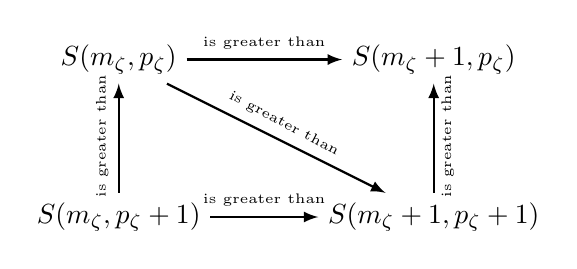
\begin{tikzpicture}
    \node[] (S00) at (0,0) {$S(m_\zeta,p_\zeta)$};
    \node[] (S10) at (4,0) {$S(m_\zeta+1,p_\zeta)$};
    \node[] (S01)  at (0,-2) {$S(m_\zeta,p_\zeta+1)$};
    \node[] (S11)  at (4,-2) {$S(m_\zeta+1,p_\zeta+1)$};
    \draw[->,thick,>=latex] (S00) -- node[anchor=south] {\tiny{is greater than}} (S10);
    \draw[->,thick,>=latex] (S01) -- node[anchor=south] {\tiny{is greater than}} (S11);
    \draw[->,thick,>=latex] (S11) -- node[anchor=west,xshift=5,yshift=-25,rotate=90] {\tiny{is greater than}} (S10);
    \draw[->, thick,>=latex] (S00) -- node[anchor=south,rotate=-28] {\tiny{is greater than}} (S11);
    \draw[->,thick,>=latex] (S01) -- node[anchor=west,xshift=-6,yshift=-25,rotate=90] {\tiny{is greater than}} (S00);
\end{tikzpicture}
\caption{Behaviour of the landscape of Surprise $S$.}
\label{fig:surprisebehaviour}
\end{figure}

A fourth inequality $S(m_\zeta,p_\zeta+1)>S(m_\zeta+1,p_\zeta)$ is implicit by looking at the behaviour of $S(\zeta)$ for a given graph. 
%\subsection{Pareto optimality}
The scheme in Figure \ref{fig:surprisebehaviour} allows to rank the values of Surprise in relation to changes in $m_\zeta$ and $p_\zeta$. It's easy  verify that $S$ satisfies the following strict order relation:
\begin{equation}\label{eq:surpriseorderrelation}
S(m_\zeta+1,p_\zeta)<S(m_\zeta+1,p_\zeta+1)<S(m_\zeta,p_\zeta)<S(m_\zeta,p_\zeta+1).
\end{equation}
This property leads us to the observation that Surprise $S$ is a monotonically decreasing function (increasing $\hat{S}$) of $m_\zeta$ and monotonically increasing function (decreasing $\hat{S}$) of $p_\zeta$ in the convex interval $\mathcal{L}$.
Moreover, from Figure \ref{fig:surprisebehaviour} follows that optimal solutions with respect to $S$ are Pareto-optimal with respect to maximizing $m_\zeta$ and minimizing $p_\zeta$.
In other words, a partition that is optimum with respect to Surprise is such that no further increment in $m_\zeta$ leads to a decrement in $p_\zeta$ that has higher $\hat{S}$.

% \begin{figure}[htb!]
% \centering
% \begin{tikzpicture}[scale=0.6, every node/.style={scale=0.6}]
% \def \S {1};
% \def \W {11};
% \def \H {7};
% \node[anchor=south west, inner sep=0mm] at (0,0) { 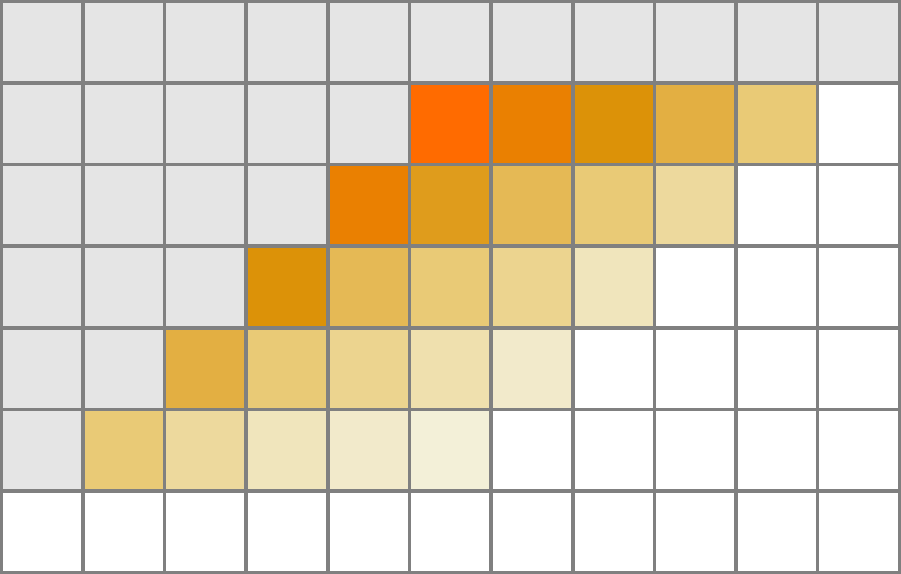
\includegraphics[width=\W cm]{images/plot_surprise_pareto.pdf}};
% \node[anchor=south] at (\W /2,\H +0.25) {$\hat{S}=-\log_{10}(S(m_\zeta,p_\zeta$, $m=10$,$p=15$))};
% %\draw[help lines,xstep=1.0,ystep=1.0] (0,0) grid (\W,\H);
% \foreach \x in {1,...,\W } {\node [anchor=north] at (\x-0.5,0) {$\x$}; }
% \node[anchor=north] at (\W/2,-0.5){$p_\zeta$};
% \foreach \y in {1,...,\H} {\node [anchor=east] at (0 ,\y-0.5) {$\y$}; }
% \node[anchor=east] at (-0.5,\H/2){$m_\zeta$};
% %\node[rectangle,fill=black!10,draw=black,rounded corners=0.1cm] at (\W+1.5,\H-0.5) {$m_{\zeta},p_\zeta \not \subset \mathcal{L}$};
% \end{tikzpicture}
% \caption{Pareto optimality of Surprise (here $\hat{S}$ is represented) on a trivial graph with $n=6$ nodes and $m=7$ edges. No increment in $m_\zeta$ leads to a decrement in $p_\zeta$ that has higher $\hat{S}$. Here Surprise is optimal for $m_\zeta=6,p_\zeta=6$.}
% \label{fig:pareto_optimality_surprise}
% \end{figure}
% \todo[inline]{CONTROLLARE FIGURA PROBABILMENTE SBAGLIATA PERCHE MZETA>M!!!}

The Pareto optimality of optimum Surprise partitions, implies that introducing a perturbation of $m_\zeta$ and $p_\zeta$ leads to a change in Surprise such that it monotonically decreases only if $\delta m_\zeta > \delta p_\zeta$, precisely:
\begin{equation}\label{eq:resolution_limit_condition}
S(m_\zeta + \delta_{m_\zeta}, p_\zeta + \delta_{p_\zeta}) < S(m_\zeta,p_\zeta) \iff \delta_{m_\zeta} \geq \delta_{p_\zeta}
\end{equation}

The result in Eq.\ref{eq:resolution_limit_condition} is of great help in designing optimization algorithms as every move that increase the intracluster edges more than intracluster pairs is good, while moves that increase intracluster pairs more than intracluster edges must be ignored, therefore sparing time for the computation of Surprise. Additionally, Eq.~\ref{eq:resolution_limit_condition} is useful when analyzing the onset of the resolution limit for different models.
In the next sections we will show to what extent Surprise is affected by the resolution limit for Surprise, to show with convincing theoretical arguments that $S$ is nearly resolution-limit-free in Traag's sense~\cite{traag2015}.


%%%%%%%%%%%%%%%%%%%%%%%%%%%%%%%%%%%%%%%%%%%%%%%%%%%%%%%%%%%%%%
%%%%%%%%%%%%%%%%%%%%%%%%%%%%%%%%%%%%%%%%%%%%%%%%%%%%%%%%%%%%%%
%%%%%%%%%%%%%%%%%%%%%%%%%%%%%%%%%%%%%%%%%%%%%%%%%%%%%%%%%%%%%%
\section{Resolution limit and Surprise}
Unfortunately, the resolution limit appears to be an intrinsic feature of many methods that optimize global quality functions, and there appears to be a ``narrow scope to resolution-limit-free methods''~\cite{traag2015}. 
Surprise has been shown to outperform other network partitioning methods in the detection of small features within large graphs, but the extent to which it suffered from the resolution limit was unknown~\cite{aldecoa2011,aldecoa2013} until our work~\cite{Nicolini2016}.

As pointed out by the authors who originally introduced Surprise~\cite{aldecoa2011}, while Modularity-based methods define a community as a region with an unexpectedly high density of links with respect to the global characteristics of the network, Surprise weights the number of actual intracluster edges against the maximum number of links given the nodes in the clusters.
Hence, Surprise is able to discriminate local subnetworks whose internal density is close to that of a clique independently of their size.
In the following, we assess the extent to which the resolution limit may affect Surprise.

In order to assess to what extent Surprise is affected by the resolution limit, we directly compared Newman's Modularity and Surprise in the example of Fortunato and Barthelemy as illustrated in the previous chapter in Figure~\ref{fig:figure_1_barthelemy}. Already for $m_{12} = 1$, i.e. when the two cliques $G_1$ and $G_2$ were connected by only one edge, $Q^N$ showed sign inversion for $m_0 \approx 200$, meaning that it was beneficial for Modularity to merge two cliques.

Surprise instead never merges cliques in the example of Fortunato and Barthelemy, as evident from Figure~\ref{fig:barthelemy_surprise}.

\begin{figure}
\centering
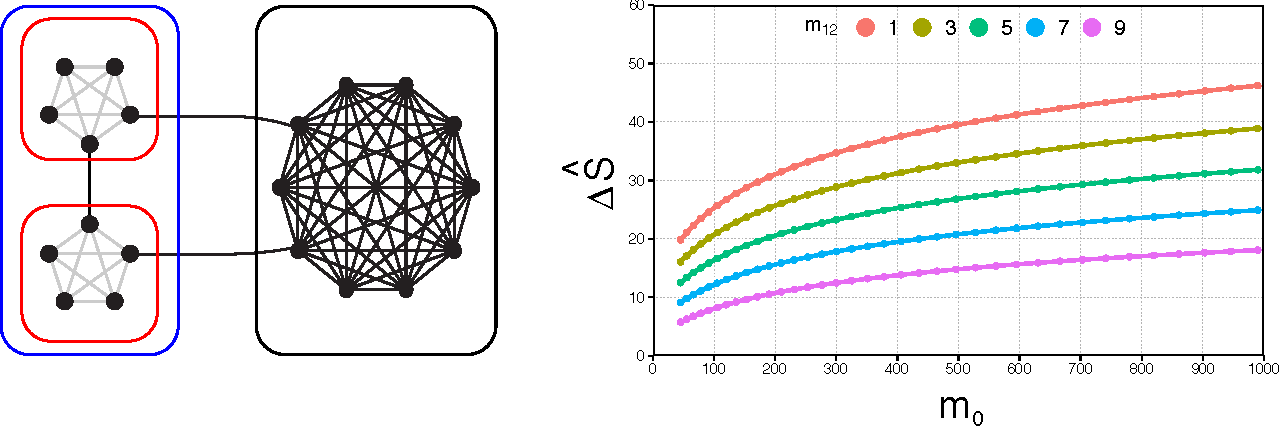
\includegraphics[width=0.8\textwidth]{images/barthelemy_surprise.pdf}
\caption{Example of a toy network with Surprise.}
\label{fig:barthelemy_surprise}
\end{figure}

Figure~\ref{fig:barthelemy_surprise} shows that Surprise does not suffer from the resolution limit at least in this specific case.
Indeed, $\Delta \hat{S}$ was always positive and grew monotonically with increasing $m_0$. 
Hence, the two cliques $G_1$ and $G_2$ were always resolved by Surprise as separate communities independently of the network size, and also in the presence of some ``fuzziness'', i.e. when $m_{12}>1$ and the two cliques were connected by more than one edge.
In order to assess whether this behavior reflects a general property of Surprise, or is incidental to this particular example, we have also studied a generalization of Fortunato and Barthelemy's model.

Traag et al.~\cite{traag2011} proposed a rigorous definition of resolution-limit-free graph partitioning.
A quality function is resolution-limit-free if, given an optimal partition $\zeta$ of a graph $G$, any module $\zeta_i$ is also optimal for the graph induced by the nodes in $\zeta_i$.
In other words, each community of the optimal partition is not split by optimization of the quality function applied to the subgraph induced by the nodes in the community.
Hence, each community does not depend on the rest of the network and is both locally and globally optimal.
An important consequence of this definition is that a resolution-limit-free method will never depend on the size of the network to merge cliques in a graph comprising $r$ cliques of $n_r$ nodes connected in a ring structure as in Figure~\ref{fig:traag_ring_of_cliques}.

This observation prompted us to explore the behavior of $\hat{S}$ in the ring of cliques model graph, as an extension of Fortunato and Barthelemy's model.
Interestingly, given its two-variables formulation, Surprise optimization can be seen as a multiobjective optimization problem where one seeks to minimize the intracluster pairs while maximizing the number of intracluster edges.
With increasing graph size, the computational problem of calculating $\hat{S}$ for every possible partition becomes rapidly intractable (maximization of $S$ is NP hard)~\cite{fleck2014}.
However, as pointed out by Fleck et al.~\cite{fleck2014}, the Surprise optimal clustering must be Pareto optimal with respect to minimizing $p_\zeta$ and maximizing $m_\zeta$, i.e. any further improvement in one of the two variables must occur at the expense of the other.

In this sense, the problem of Surprise optimization is equivalent to a linear program, where one seeks to minimize $p_\zeta$ while keeping $m_\zeta$ equal to a constant $h$, choosing among the resulting clustering, the one that maximizes $\hat{S}$.
Hence, to delineate the Pareto frontier in the $m_\zeta,p_\zeta$ space, we need to solve $m$ integer linear programs (ILP) in the form:
\begin{align}
\textrm{minimize} \sum_{\{i,j\} \in \binom{V}{2}} \mathcal{X}_{ij} \nonumber \\
\textrm{s.t.} \quad \mathcal{X}_{ij} \in \{0,1 \} \nonumber \\
\quad \mathcal{X}_{ik} + \mathcal{X}_{ki} - \mathcal{X}_{ij} \leq 1 \nonumber \\
\sum_{\{i,j\} \in E} \mathcal{X}_{ij}=h \nonumber
\end{align}
where $\mathcal{X}_{ij}$ are a set of $\binom{n}{2}$ binary variables corresponding to vertex pairs, with the interpretation that $\mathcal{X}_{ij}=1$ if vertex $i$ and vertex $j$ are in the same community.
The constraint are necessary in order to ensure that if node $i$ and node $j$ are in the same community and node $i$ and node $k$ are in the same community, then node $j$ and node $k$ are in the same community too.

%where we sought to minimize $p_\zeta$ while keeping $m_\zeta$ equal to a constant $h$, with $\mathcal{h}$ ranging from $0$ (trivial partition where every vertex is a community) to $m$ (trivial partition with all vertices in the same community).
 Linear programs were solved using the Python interfaces of Gurobi 5.7.3 on Linux (Gurobi Optimizer Version 5.7, Gurobi Optimization, Inc., Houston, Texas, United States).

Figure 2B shows the Pareto frontier for a ring of cliques where we independently varied the number of cliques $r$ and the number of nodes $n$ in every clique.
Interestingly, $\hat{S}$ increased monotonically along the Pareto frontier with increasing $p_\zeta$ (Fig. 2C), until it reached its optimum, indicated by black circles in the Pareto frontier, for the partition that identi ed each clique as a separate community.
Importantly, in the range of parameters we have investigated, Surprise optimization never merged cliques in the ring of cliques, independently of the size of the graph, and behaved as a Traag's resolution-limit free method.
While it is likely that this property is quite general and can be extended to every ring of cliques, an analytical demonstration is hampered by the non-additivity of the Surprise function.
Nonetheless, the size of the graphs we have explored numerically is quite typical of brain-connectivity networks and we feel encouraged to apply Surprise maximization to the study of the community structure of the brain.


%%%%%%%%%%%%%%%%%%%%%%%%%%%%%%%%%%%%%%%%%%%%%%%%%%%%%%%%%%%%
%%%%%%%%%%%%%%%%%%%%%%%%%%%%%%%%%%%%%%%%%%%%%%%%%%%%%%%%%%%%
%%%%%%%%%%%%%%%%%%%%%%%%%%%%%%%%%%%%%%%%%%%%%%%%%%%%%%%%%%%%
\subsection{Statistical test}\label{sec:surprisefishertest}
Surprise considers the problem of community detection as the one of making the intracluster density as different as possible from the global density in statistical terms. In this sense, it's worth noting that $S$ is \emph{p}-value of a one-tailed Fisher exact-test where one is asking how confidently should reject the null hypothesis $H_0$ that the intracluster density is the same as the graph density.
It turns indeed out that this problem has an equivalent description in statistics, where one seeks to maximize the \emph{odds-ratio} of the $2 \times 2$ contingency table defined in Table~\ref{tab:contingency_table}.
\begin{table}[htb!]
\centering
\begin{tabular}{|c|c|c|c|}
\hline
 & Drawn & Not drawn & \textbf{Total}\\
\hline
Intracluster & $m_\zeta$ & $p_\zeta-m_\zeta$ & $p_\zeta$\\
\hline
Intercluster & $m-m_\zeta$ & $p-m-p_\zeta+m_\zeta$ & $p-p_\zeta$ \\
\hline
\textbf{Total} & $m$ & $p-m$ & $p$ \\
\hline
\end{tabular}
\caption{Contingency table for the urn model.}
\label{tab:contingency_table}
\end{table}
The Fisher exact test implemented by Surprise is, as its name states, exact as long as the contingency table keeps the row and column totals fixed, and it can therefore be used regardless of the sample characteristics. A simpler $\chi^2$ statistic can be used when the elements of the contingency table are large enough, although only an approximation of the \emph{p}-value can be obtained.
In this case it's possible to tackle the problem of computation of $S$ by means of odds-ratio. Precisely, the \emph{normalized log odds-ratio} is computed as 
\begin{equation}
\log(\textrm{OR}) = \log\left( \frac{m_\zeta(p-m-p_\zeta+m_\zeta)}{(m-m_\zeta)(p_\zeta-m_\zeta)} \right )
\end{equation}
and in the asymptotic case, Surprise is equal to the probability:
\begin{equation}
\Pr\left(z < -\frac{|\log\textrm{OR})|}{SE} \right)
\end{equation}
where $z$ is a random variable with standard normal distribution $z \approx \mathcal{N}(0,1)$.

Although of almost null interest for the case of binary graphs, this last equation is telling us that in developing a version of Surprise that will keep into account weighted graphs, we should in some way rely on its asymptotic distribution.